\section{section title}
\begin{frame}
  \frametitle{Why do we need manipulation-based search for occluded
    objects?}
  \begin{figure}
    \centering
    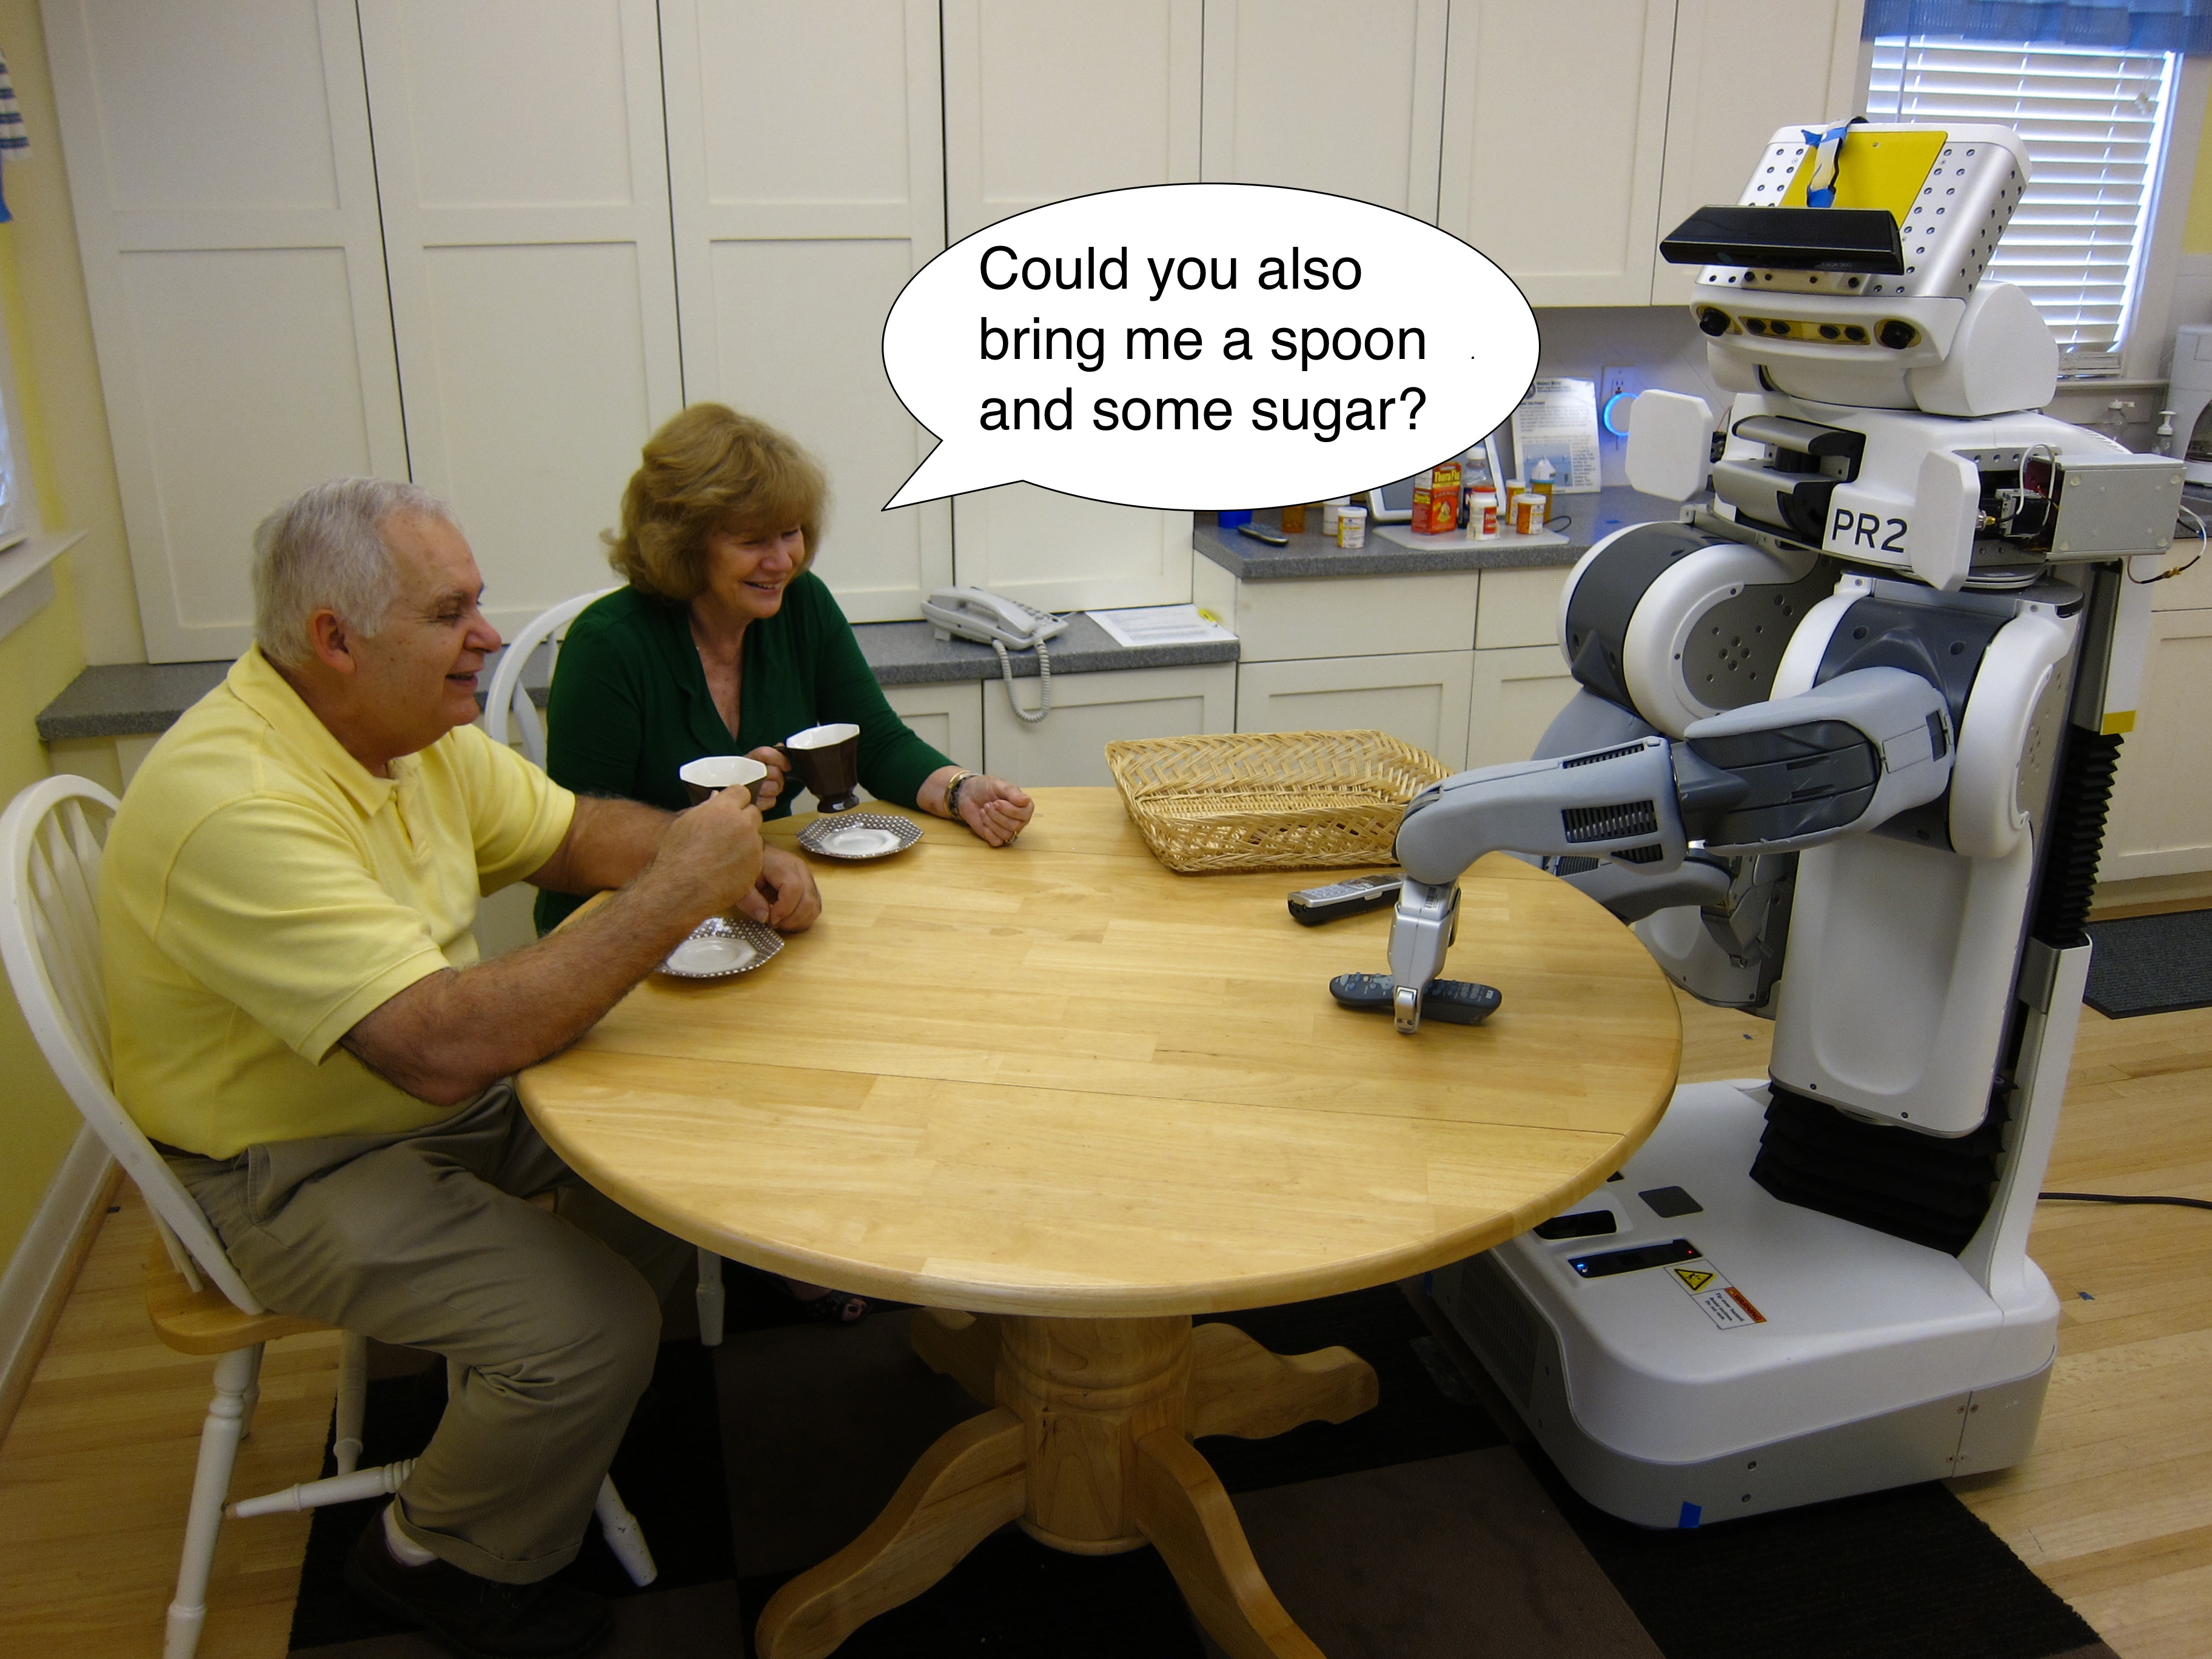
\includegraphics[width=3.2in]{img/robot_in_kitchen.jpg}

    \tiny{Original image courtesy of Wendy Rogers/Georgia Tech}
  \end{figure}
\end{frame}

\begin{frame}
  \frametitle{Assumptions for the following treatment}
  \begin{itemize}
  \item No errors in  visual identification and classification of objects
  \item Robot can successfully complete any movement and manipulation task, but
    these are temporally expensive
  \item Finite set of object types in the world
  \end{itemize}
\end{frame}
